%%%%%%%%%% Merge with supplemental materials %%%%%%%%%%
\pagebreak
% \widetext
\begin{center}
\textbf{\large Supplementary Material for Hemodynamic Deconvolution Demystified: Sparsity-Driven Regularization at Work}
\end{center}
%%%%%%%%%% Merge with supplemental materials %%%%%%%%%%
%%%%%%%%%% Prefix a "S" to all equations, figures, tables and reset the counter %%%%%%%%%%
\setcounter{equation}{0}
\setcounter{figure}{0}
\setcounter{table}{0}
\setcounter{page}{1}
\makeatletter
\renewcommand{\theequation}{S\arabic{equation}}
\renewcommand{\thefigure}{S\arabic{figure}}
\renewcommand{\bibnumfmt}[1]{[S#1]}
\renewcommand{\citenumfont}[1]{S#1}
%%%%%%%%%% Prefix a "S" to all equations, figures, tables and reset the counter %%%%%%%%%%

\begin{figure*}[h!]
    \begin{center}
        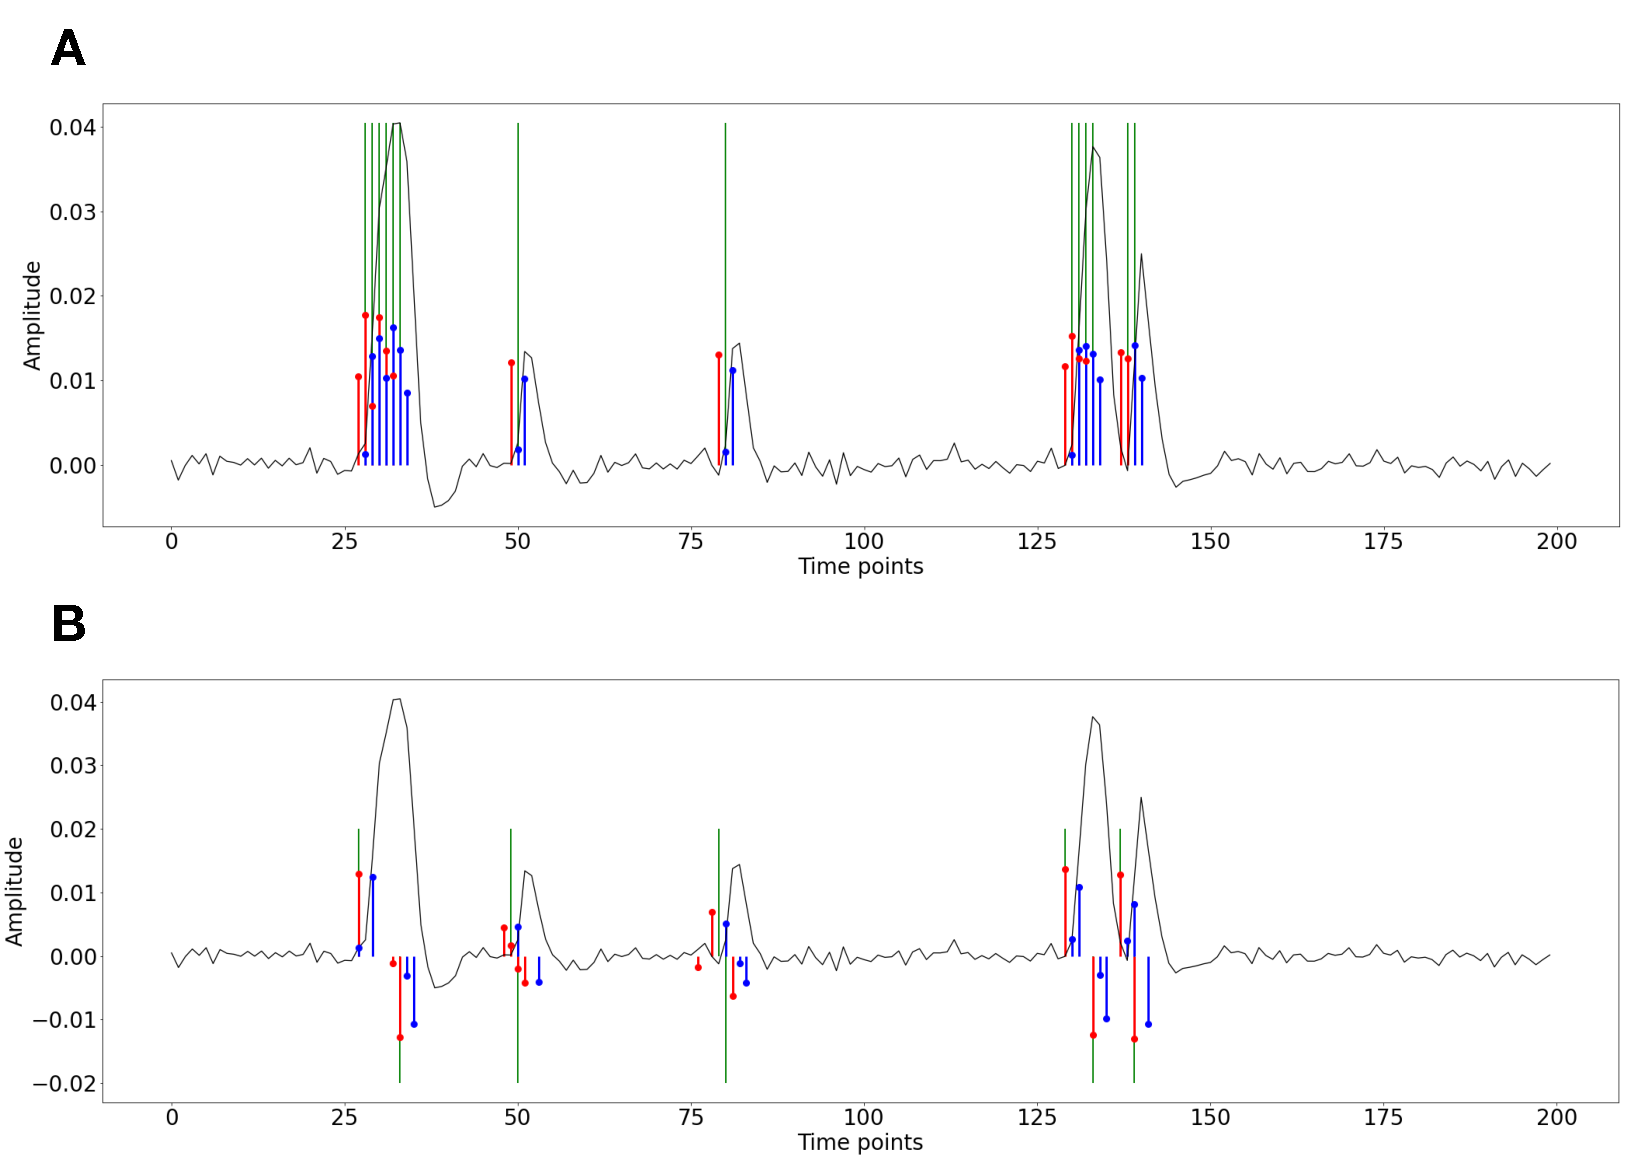
\includegraphics[width=\textwidth]{figures/supp_hrf_differences.pdf}
    \end{center}
    \caption{}
\label{fig:hrf_differences}
\end{figure*}

\begin{figure*}[h!]
    \begin{center}
        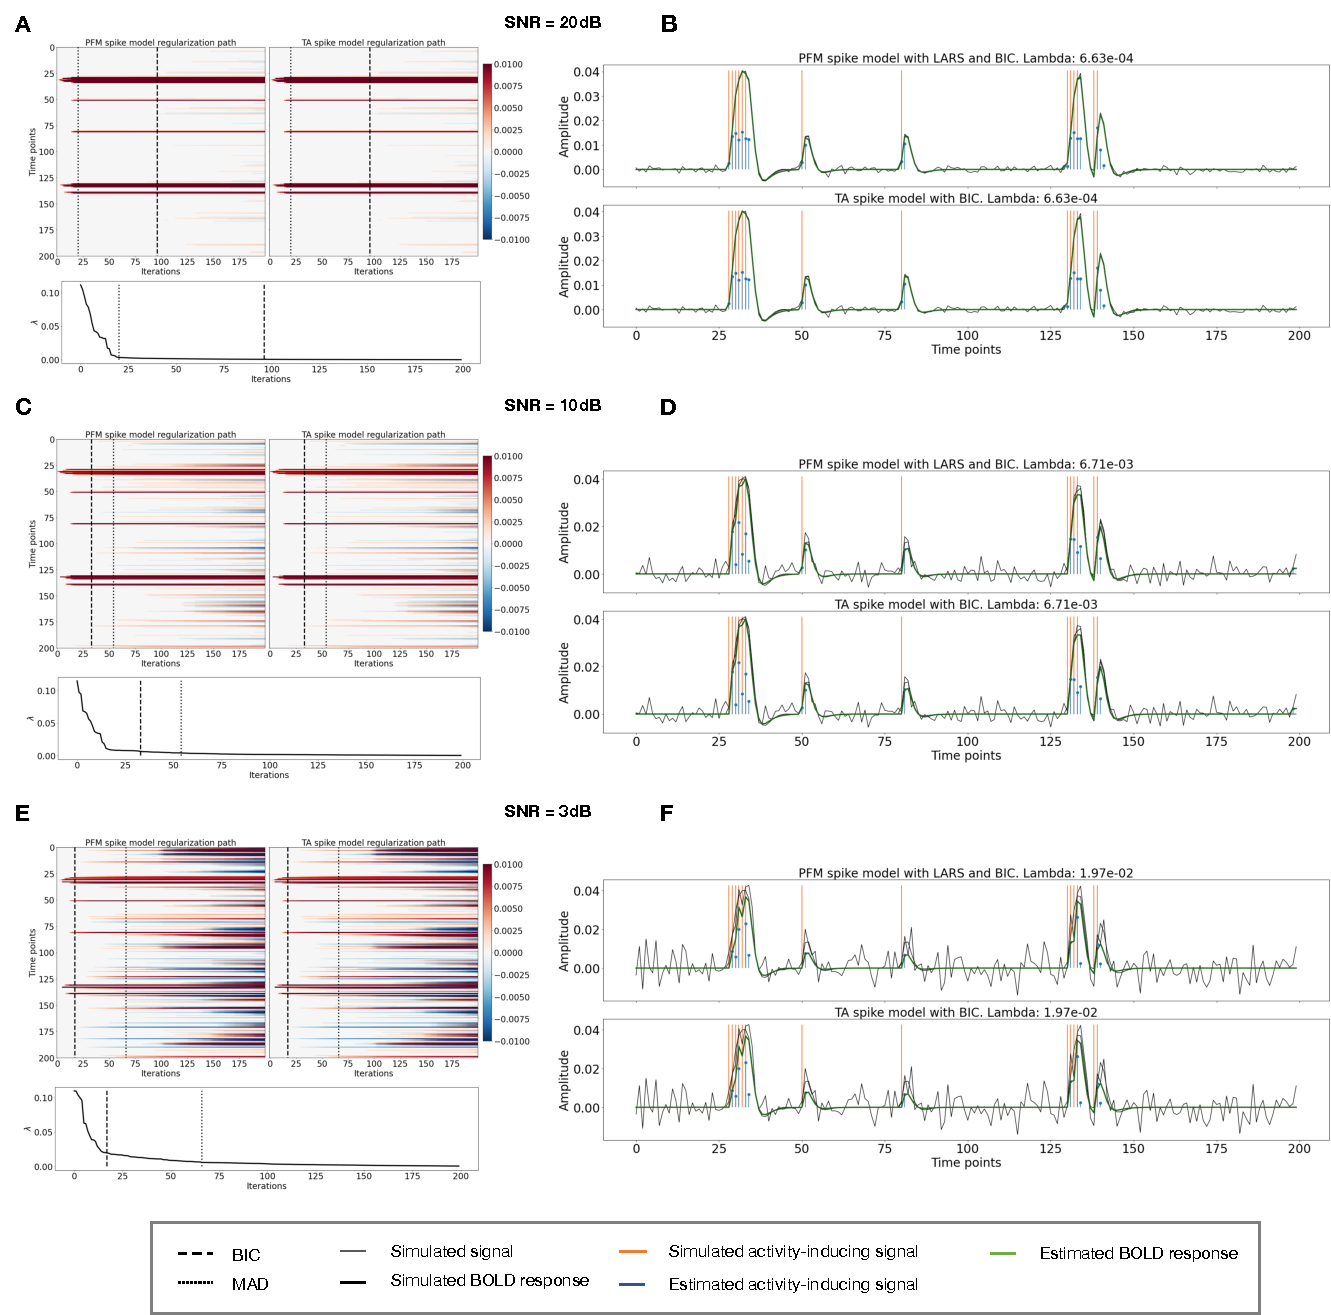
\includegraphics[width=\textwidth]{figures/regpath_spike.pdf}
    \end{center}
    \caption{Spike model simulations. (Left) Heatmap of the regularization paths of the activity-inducing signal estimated with PFM and TA as a function of \(\lambda\) (increasing number of iterations in x-axis), whereas each row in the y-axis shows one time-point. Vertical lines denote iterations corresponding to the Akaike and Bayesian Information Criteria (AIC and BIC) optima. (Right) Estimated activity-inducing (blue) and activity-related (green) signals when set based on BIC. All estimates of are identical, regardless of SNR.}
\label{fig:path_spike}
\end{figure*}

\begin{figure*}[h!]
    \begin{center}
        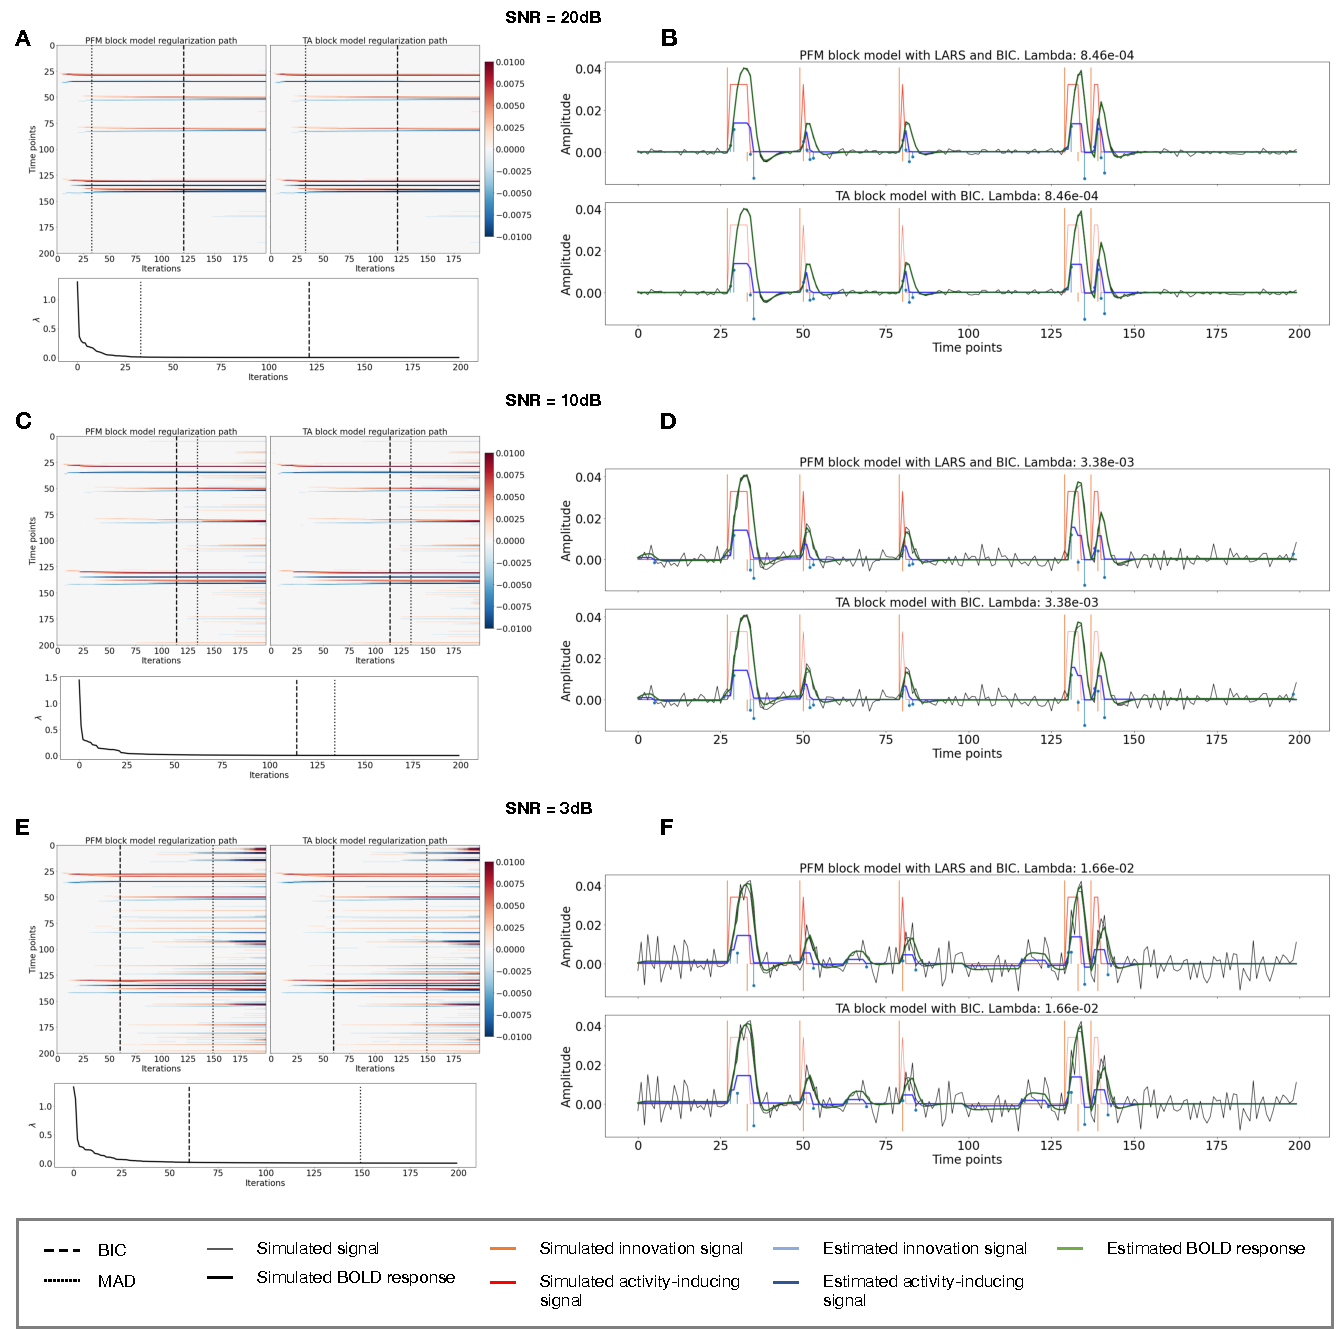
\includegraphics[width=\textwidth]{figures/regpath_block.pdf}
    \end{center}
    \caption{Block model simulations. (Left) Heatmap of the regularization paths of the innovation signal estimated with PFM and TA as a function of \(\lambda\) (increasing number of iterations in x-axis), whereas each row in the y-axis illustrates one time-point. Vertical lines denote iterations corresponding to the Akaike and Bayesian Information Criteria (AIC and BIC) optima. (Right) Estimated innovation (blue) and activity-related (green) signals when is set based on BIC. All the estimates are identical when compared between the PFM and TA cases, regardless of SNR.}
\label{fig:path_block}
\end{figure*}

% \begin{figure*}[h!]
%     \begin{center}
%         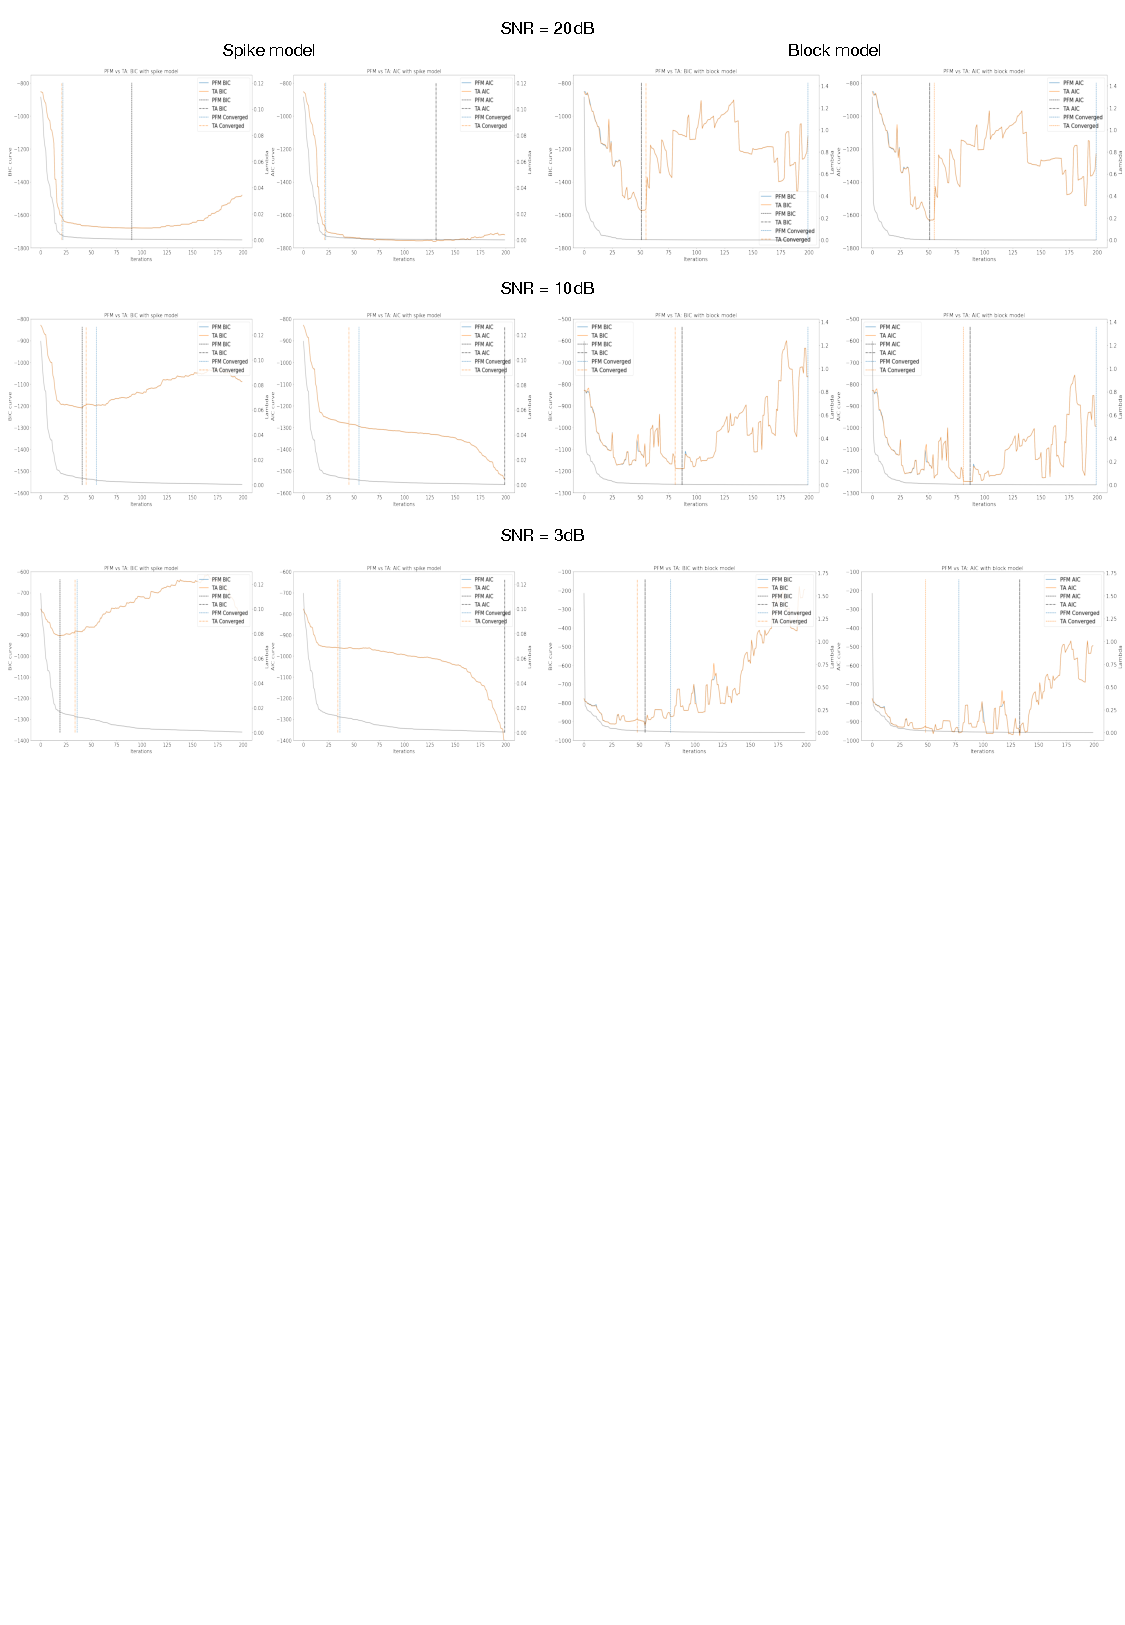
\includegraphics[width=\textwidth]{figures/lambda_cost.pdf}
%     \end{center}
%     \caption{Lambdas and cost.}
% \label{fig:lambdas}
% \end{figure*}

\begin{figure*}[h!]
    \begin{center}
        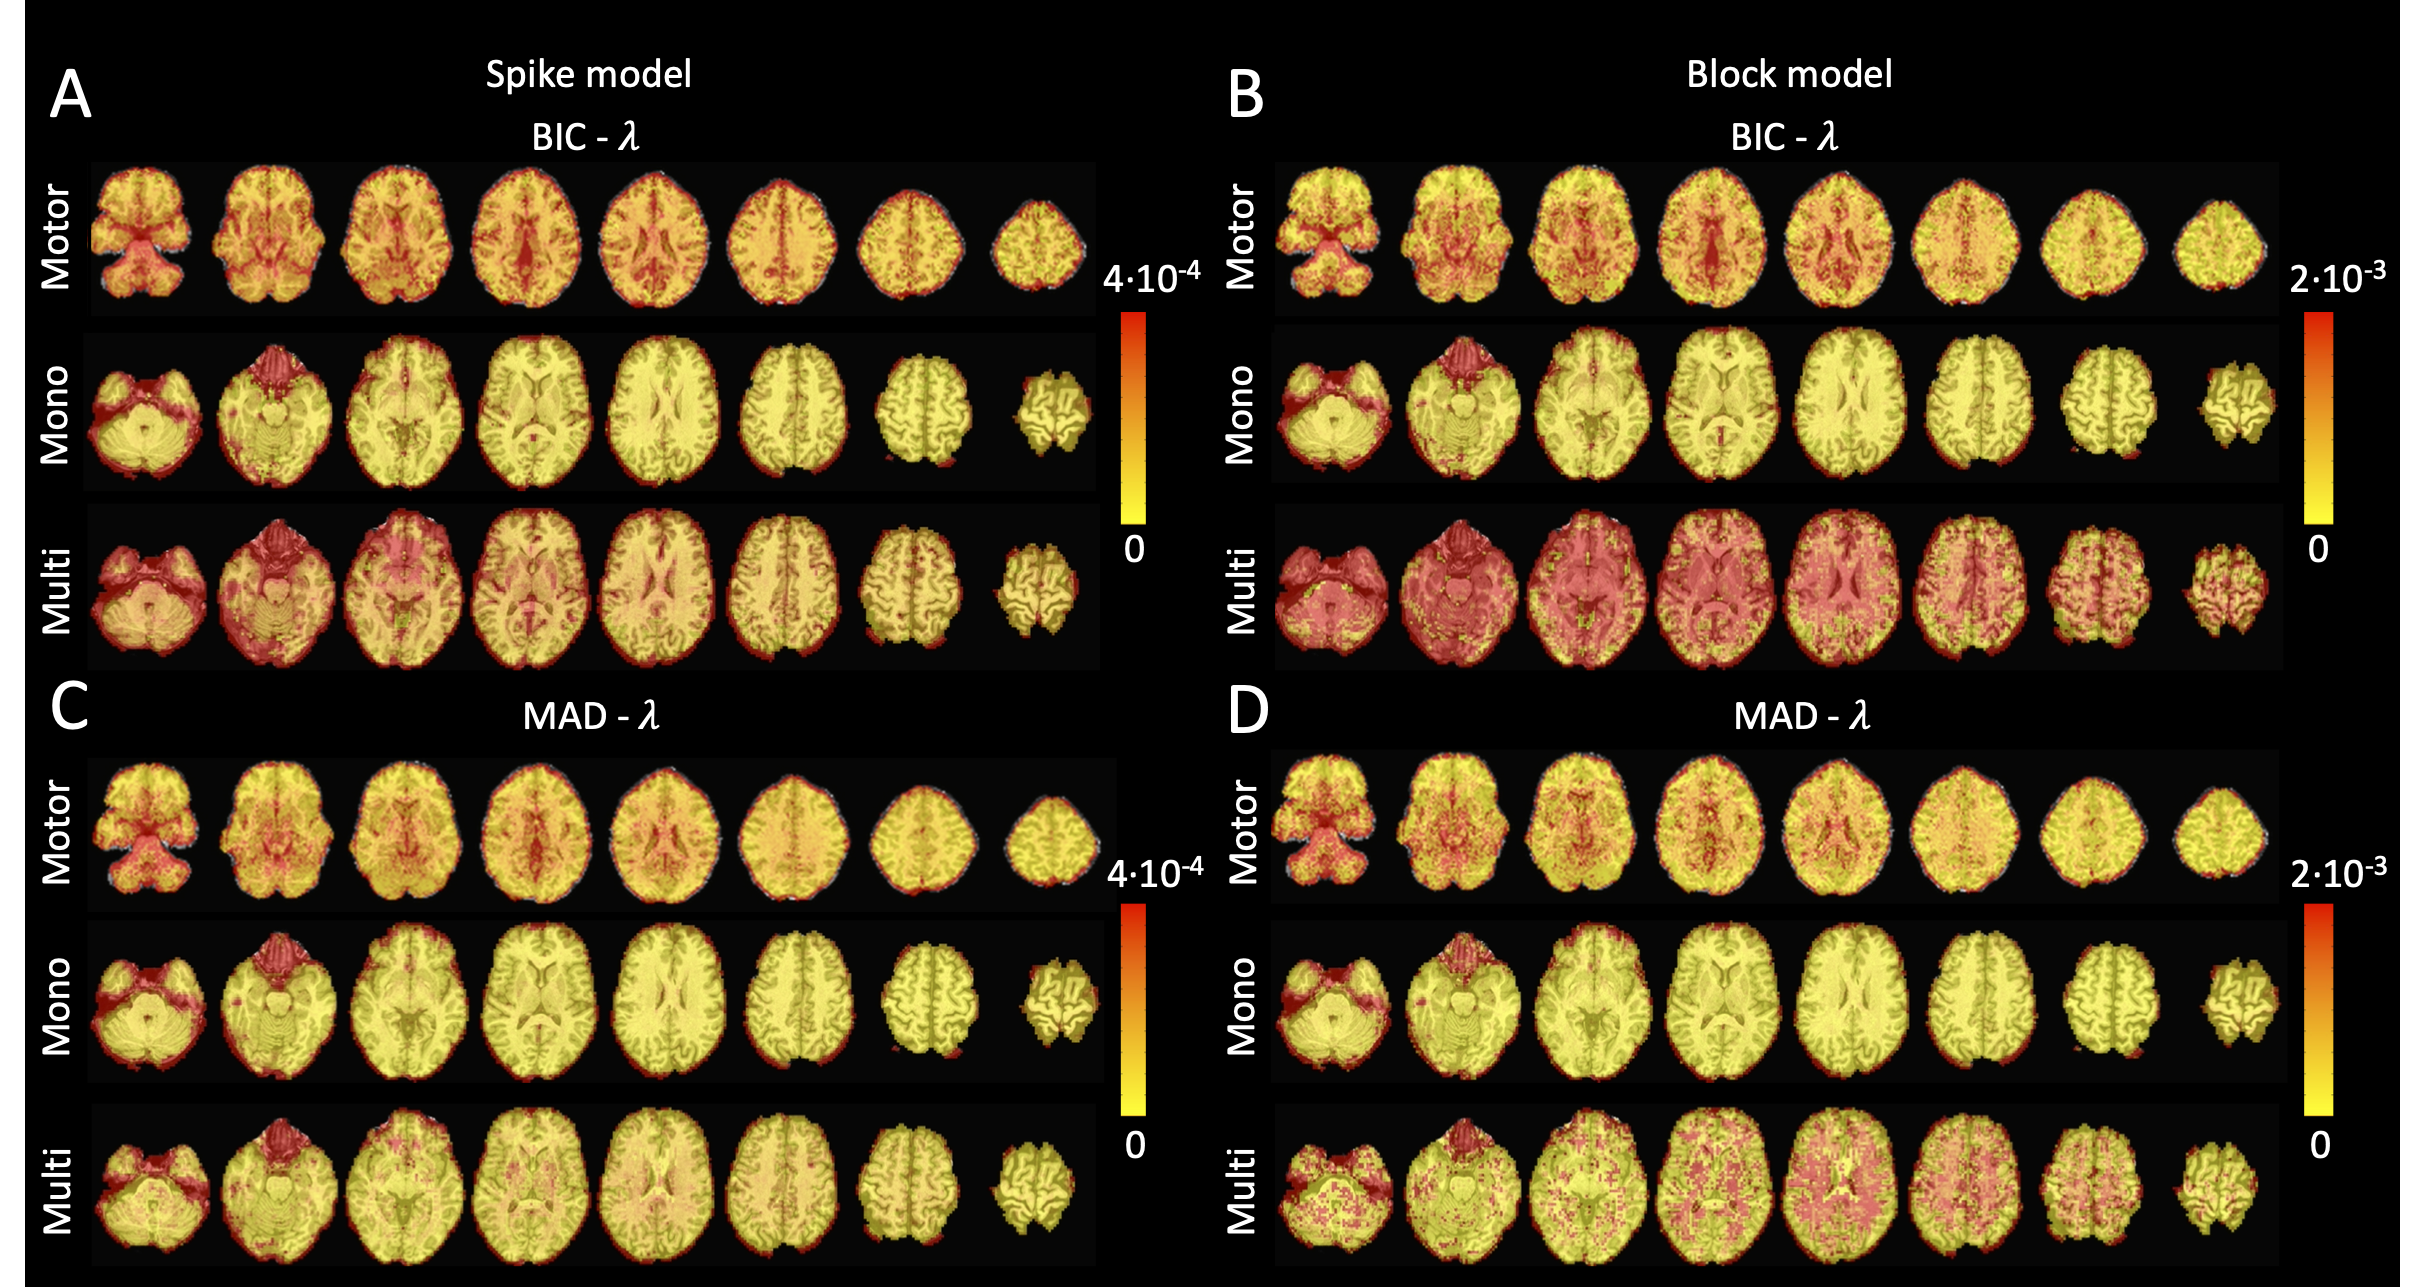
\includegraphics[width=\textwidth]{figures/supp_lambdas_map.pdf}
    \end{center}
    \caption{Values of $\lambda$ across the different voxels in the brain used to estimate (A) the activity-inducing signal (spike model) and (B) the innovation signal (block model) with the BIC selection, as well as (C) the activity-inducing signal (block model) and (D) the innovation signal (block model) with a MAD-based selection. The $\lambda$ maps are shown for the three experimental fMRI datasets: the motor task (Motor), the monoband resting-state (Mono), and the multiband resting-state (Multi) datasets.}
\label{fig:lambdas}
\end{figure*}

\begin{figure*}[h!]
    \begin{center}
        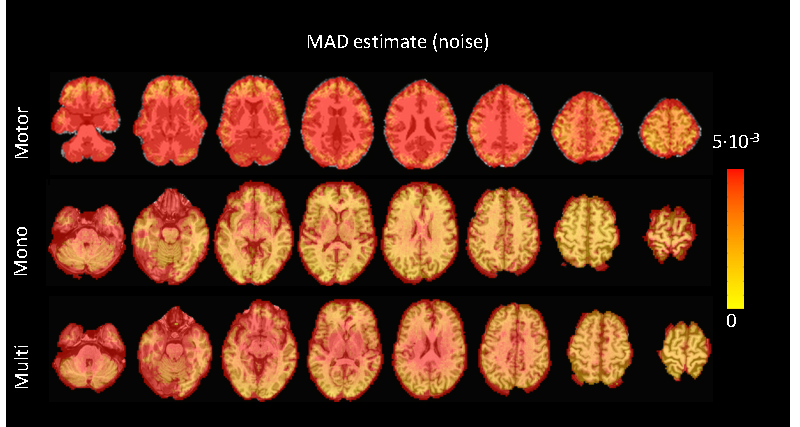
\includegraphics[width=\textwidth]{figures/supp_mad_estimate.pdf}
    \end{center}
    \caption{Values of the MAD estimate of standard deviation of the noise across the different voxels in the brain for the three experimental fMRI datasets: the motor task (Motor), the monoband resting-state (Mono), and the multiband resting-state (Multi) datasets.}
\label{fig:mad_estimate}
\end{figure*}

\begin{figure*}[h!]
    \begin{center}
        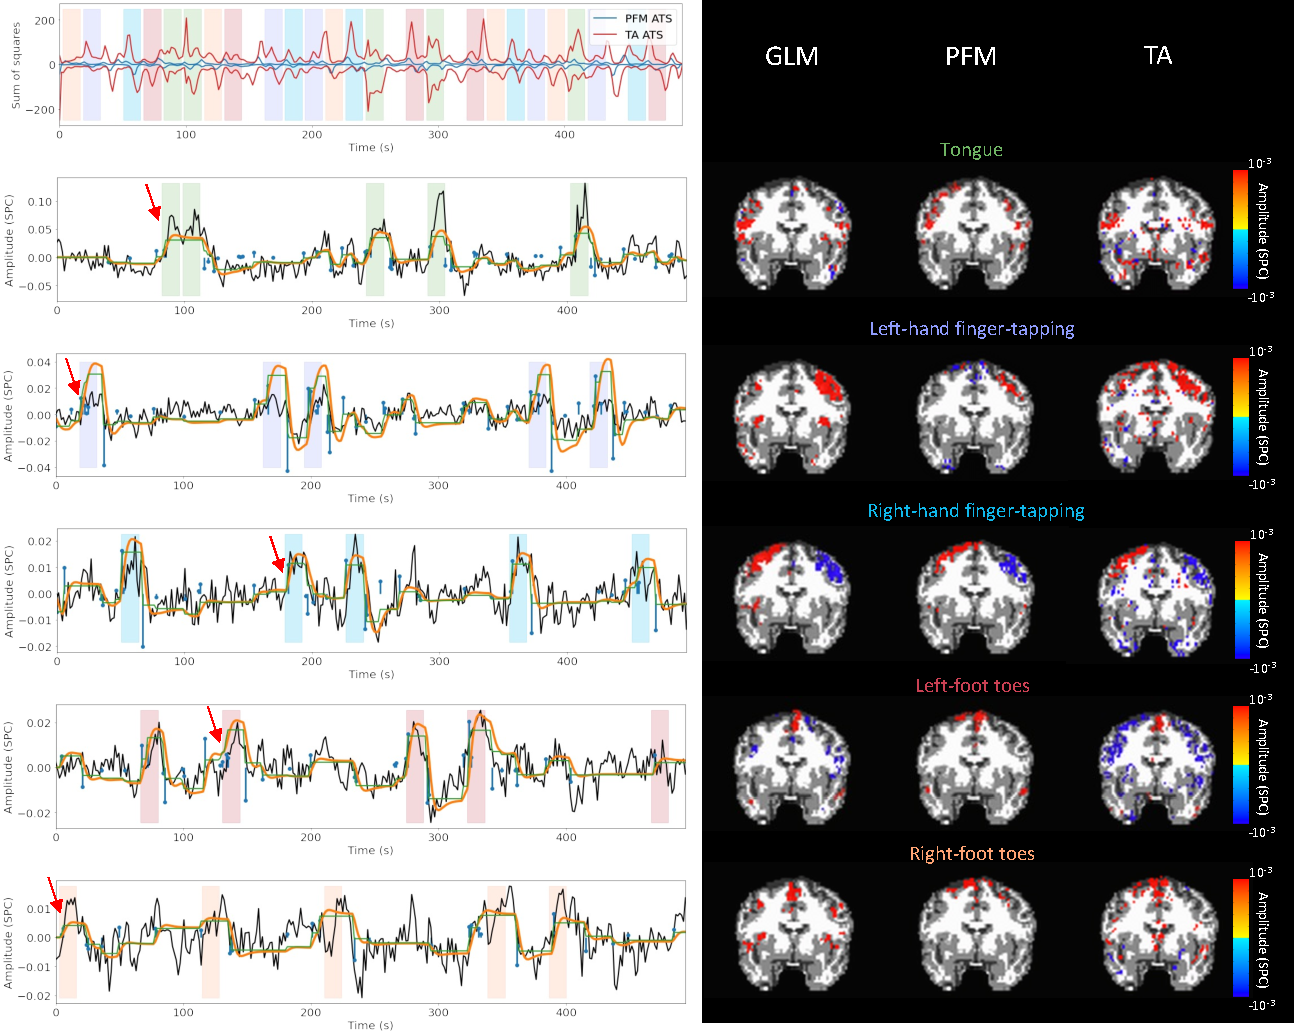
\includegraphics[width=\textwidth]{figures/supp_task_maps_mad.pdf}
    \end{center}
    \caption{Activity maps of the motor task using a seletion of $\lambda$ based on the MAD estimate. Row 1: Activation time-series of the innovation signals estimated by PFM (in blue) or TA (in red) calculated as the sum of squares of all voxels at every timepoint. Positive-valued and negative-valued contributions were separated into two distinct time-courses. Color-bands indicate the onset and duration of each condition in the task (green: tongue, purple: left-hand finger-tapping, blue: right-hand finger-tapping, red: left-foot toes, orange: right-foot toes). Rows 2-6: time-series of a representative voxel for each task with the PFM-estimated innovation (blue), PFM-estimated activity-inducing (green), and activity-related (i.e., fitted, orange) signals, with their corresponding GLM, PFM, and TA maps on the right. The maps shown on the right are sampled at the time-point labeled with the red arrows and display the innovation signals at that moment across the whole brain.}
\label{fig:task_mad}
\end{figure*}

\begin{figure*}[h!]
    \begin{center}
        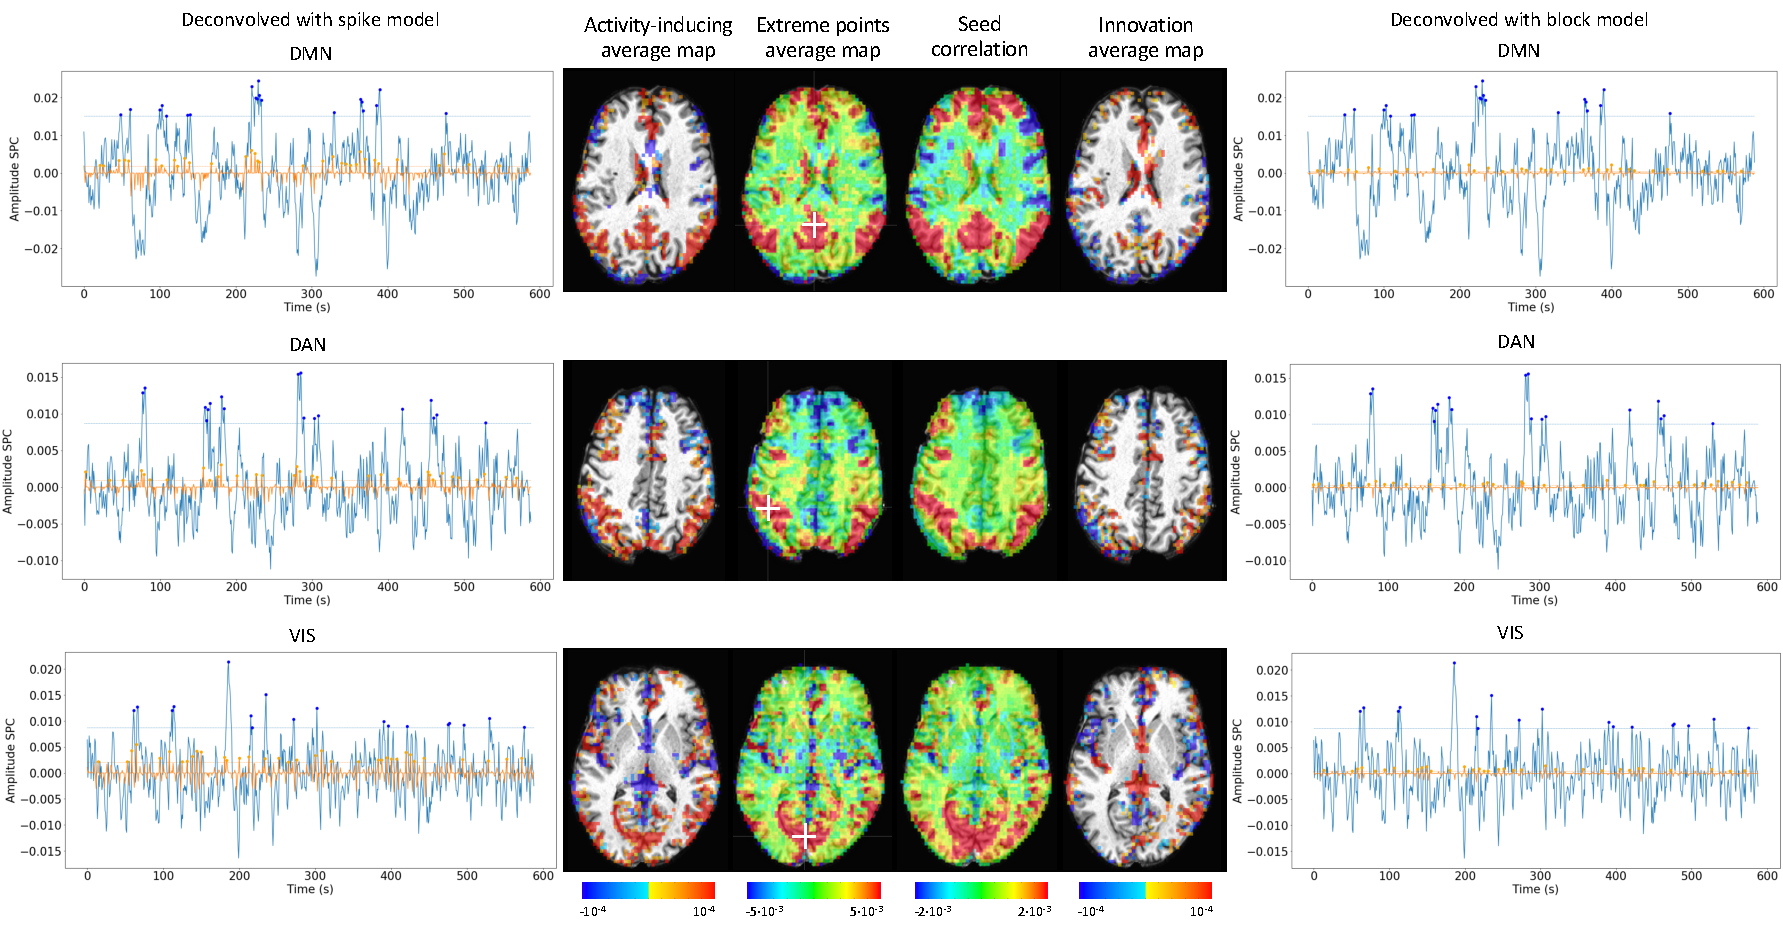
\includegraphics[width=\textwidth]{figures/supp_caps_mad.pdf}
    \end{center}
    \caption{Activity-inducing CAPs (left) and innovation CAPs (right) obtained with the PFM-estimated activity-inducing and innovation signals respectively, using a MAD-based selection of $\lambda$. Time-points selected with a 95th percentile threshold are shown over the average time-series (blue) in the seed region (white-cross) and the deconvolved signal (orange). CAPs and seed correlation maps are illustrated in the center.}
\label{fig:caps_mad}
\end{figure*}